\documentclass[../../FisicaTeorica.tex]{subfiles}
\begin{document}
\subsection{Barriera di potenziale}
Consideriamo ora il caso di una \textit{barriera di potenziale} data da $V(x)=\bar{V}\chi_{\left[-\frac{a}{2},\frac{a}{2}\right]}$
%[IMMAGINE] potenziale a gradino di altezza \bar{V} tra -a/2 e a/2, e nullo altrimenti. Evidenziati le regioni 1 (partenza), 2 (gradino), 3 (uscita)
L'effetto quantistico più rilevante si ha per $\mathcal{E}<\bar{V}$. In tal caso l'onda evanescente di probabilità vista nel gradino dà luogo all'\textbf{effetto tunnel}\index{Effetto tunnel}, cioè a una probabilità finita di trovare la particella che proviene dalla regione 1 nella regione 3, passando in una regione 2 proibita classicamente (energia cinetica $<0$).\\

Nella risoluzione partiamo tuttavia dal caso $\mathcal{E}>\bar{V}$, che potremo poi adattare a quello $\mathcal{E}<\bar{V}$ che ci interessa.\\
\paragraph{Energia più alta del gradino\\}\marginpar{Caso: $\bm{\mathcal{E}>\bar{V}}$}
Se $\mathcal{E}>\bar{V}$ la soluzione dell'equazione agli autovalori è, nelle regioni $1$ e $2$ esattamente la stessa già trovata per il gradino, mentre la regione $3$ è analoga alla $1$, visto che in entrambe $V(x)=0$. Si ha quindi:
\marginpar{1. Autofunzioni $\varphi_{\mathcal{E}>\bar{V}}(x)$}
\begin{equation}
\varphi_\mathcal{E}(x)= \begin{cases}
c^1_+ e^{ik_1x} + c^1_-e^{-ik_1x} & x<-\frac{a}{2}\quad (1)\\
c^2_+ e^{ik_2x}+c^2_- e^{-ik_2x} & -\frac{a}{2}<x<\frac{a}{2}\quad (2)\\
c^3_+ e^{ik_3 x} + c^3_- e^{-ik_3 x} & x>\frac{a}{2}\quad(3)
\end{cases}
\label{eqn:autofunzioni_rettangolari}
\end{equation}
con:
\[
\bm{k_1}=\frac{\sqrt{2m\mathcal{E}}}{\hbar}; \quad \bm{k_2}=\frac{\sqrt{2m(\mathcal{E}-\bar{V})}}{\hbar}; \quad k_3 = k_1
\]
Avremo\marginpar{2. Raccordo delle soluzioni} quindi due condizioni di \textbf{raccordo}, una in $-\frac{a}{2}$ e una in $\frac{a}{2}$, che vanno applicate sia per $\varphi_\mathcal{E}$ che per la derivata $\varphi'_\mathcal{E}$, per un totale di $4$ equazioni di raccordo. Dato che nella soluzione compaiono $6$ costanti, la \textbf{degenerazione} degli autovalori sarà $6-4=\bm{2}$.\\
L'equazione di raccordo a $-\frac{a}{2}$ è:
\[
\begin{cases}
\varphi_\mathcal{E}(-\frac{a}{2}^-)=\varphi_\mathcal{E}(-\frac{a}{2}^+)\\
\varphi'_\mathcal{E}(-\frac{a}{2}^-)=\varphi_\mathcal{E}(\frac{a}{2}^+)
\end{cases} \Rightarrow 
\begin{cases}
c^1_+ e^{-ik_1\frac{a}{2}}+c^1_- e^{+ik_1\frac{a}{2}}=c^2_+ e^{-ik_2\frac{a}{2}}+c^2_- e^{ik_2 \frac{a}{2}}\\
\cancel{i}k_1(c^1_+ e^{-ik_1\frac{a}{2}}-c^1_-e^{ik_1\frac{a}{2}})
=\cancel{i}k_2(c^2_+e^{-ik_2\frac{a}{2}}-c^2_-e^{ik_2\frac{a}{2}})
\end{cases}
\]
Dividendo la seconda equazione per $k_2$, per poi sommare/sottrarre membro a membro, si possono ricavare $c^2_+$ e $c^2_-$:
\begin{equation}
\begin{cases}
2c^2_+ = c^1_+\left(1+\frac{k_1}{k_2}\right) e^{i\frac{a}{2}(k_2-k_1)}+c^1_- \left(1-\frac{k_1}{k_2}\right) e^{i\frac{a}{2}(k_2+k_1)}\\
2c^2_- = c^1_+\left(1-\frac{k_1}{k_2}\right)e^{-i\frac{a}{2}(k_2+k_1)} + c^1_- \left(1+\frac{k_1}{k_2}\right) e^{-i\frac{a}{2}(k_2-k_1)}
\end{cases}
\label{eqn:raccordo1}
\end{equation}
Possiamo allora riscrivere il sistema in forma matriciale:
\begin{equation}
\begin{pmatrix}
c^2_+\\
c^2_-
\end{pmatrix} =
M \begin{pmatrix}
c^1_+\\
c^1_-
\end{pmatrix}
\label{eqn:matrice1}
\end{equation}
dove $M$ è una matrice $(2\times 2$) data da:

\begin{align*}%Questo fattore 1/2 può essere incluso nelle costanti?
\bm{M}=\frac{1}{2}\begin{pmatrix}
\left(1+\frac{k_1}{k_2}\right)e^{i(k_2-k_1)\frac{a}{2}} & \left (
1-\frac{k_1}{k_2}
\right)
e^{i(k_2+k_1)\frac{a}{2}}\\
\left(1-\frac{k_1}{k_2}\right)e^{-i(k_2+k_1)\frac{a}{2}} & \left(1+\frac{k_1}{k_2}\right)e^{-i(k_2-k_1)\frac{a}{2}}
\end{pmatrix}
\end{align*}
Per quanto riguarda le equazioni di raccordo per $\frac{a}{2}$ basta riadattare quanto ottenuto, partendo dal cambiare il segno alle $a$, ossia sostituendo $a\leftrightarrow -a$ nelle (\ref{eqn:raccordo1}). Nel nuovo caso avremo le $c^2_\pm$ a sinistra, e le $c^3_\pm$ a destra.\\
 Essendo però $k_3 = k_1$, stavolta $k_2$ compare a sinistra e $k_1$ compare a destra: ciò non è altro che il caso \textit{simmetrico} a prima, e quindi nelle (\ref{eqn:raccordo1}) basta scambiare $k_1 \leftrightarrow k_2$.\\
Possiamo perciò porre anche questo sistema in forma matriciale (stiamo sempre ricavando i termini a destra, che in questo caso sono le $c^3_\pm$:
\begin{equation}
\begin{pmatrix}
c^3_+\\
c^3_-
\end{pmatrix}
= M'
\begin{pmatrix}
c^2_+\\
c^2_-
\end{pmatrix}
\label{eqn:matrice2}
\end{equation}
dove la matrice $M'$ si ottiene da $M$ dalle sostituzioni elencate di sopra:
\[
\bm{M'}=M[a\leftrightarrow -a, k_2 \leftrightarrow k_1]
\]
Combinando (\ref{eqn:matrice1}) e (\ref{eqn:matrice2}) otteniamo:
\begin{equation}
\begin{pmatrix}
c^3_+\\
c^3_-
\end{pmatrix} = M'M\begin{pmatrix}
c^1_+\\
c^1_-
\end{pmatrix}; \quad \begin{pmatrix}
c^1_+\\
c^1_-
\end{pmatrix}=(M'M)^{-1}\begin{pmatrix}
c^3_+\\
c^3_-
\end{pmatrix}
\label{eqn:matrice3}
\end{equation}
Che è la relazione che ci interessa, dato che il nostro obiettivo finale sarà quello di calcolare i coefficienti di \textit{trasmissione} e \textit{riflessione}, in modo da confrontare il comportamento del sistema con l'analogo classico, e perciò non ci interessa il comportamento della regione di mezzo, ma solo ciò che avviene prima o dopo di essa.\\
\\
Le costanti\marginpar{Calcolo veloce di $M'M$ e $(M'M)^{-1}$} che ci servono possono essere ricavate dalle relazioni (\ref{eqn:matrice3}), ma farlo direttamente è una procedura lunga e tediosa. Possiamo di gran lunga semplificarla notando che se $\varphi_\mathcal{E}(x)$ è soluzione dell'equazione agli autovalori:
\[
H\varphi_\mathcal{E}(x)=\mathcal{E}\varphi_\mathcal{E}(x)
\]
Allora (essendo $H$ autoaggiunto e $\mathcal{E}$ reale), anche $\varphi_\mathcal{E}^*(x)$ è soluzione:
\[
H\varphi_\mathcal{E}^*(x)=\mathcal{E}\varphi_\mathcal{E}^*(x)
\]
Nel caso in questione vi è una particolare \textit{simmetria} tra le due soluzioni complesse-coniugate. Se calcoliamo $\varphi_\mathcal{E}^*(x)$:
\begin{align*}
\varphi_\mathcal{E}^*(x)&= (\hlc{Yellow}{c^1_+} e^{ik_1 x} + \hlc{SkyBlue}{c_-^1 }e^{-ik_1x})^* = c^{1*}_+ e^{-ik_1x}+c^{1*}_- e^{ik_1x} =\\
&= (\hlc{Yellow}{c^{1*}_-} e^{ik_1x}+\hlc{SkyBlue}{c^{1*}_+} e^{-ik_1 x})
\end{align*} 
Notiamo che possiamo passare da $\varphi_\mathcal{E}(x)$ alla coniugata $\varphi_\mathcal{E}^*(x)$ semplicemente sostituendo i parametri evidenziati:
\begin{equation}
c^1_+ \leftrightarrow c^{1*}_- \quad c^1_- \leftrightarrow c^{1*}_+
\label{eqn:sostituzioni_coniugate}
\end{equation}
Ciò ci permette di usare (\ref{eqn:matrice1}), (\ref{eqn:matrice2}), (\ref{eqn:matrice3})  sia per $\varphi_\mathcal{E}(x)$ che per $\varphi_\mathcal{E}^*(x)$ mantenendo le \textbf{stesse}  matrici $M$ e $M'$ in entrambi i casi, e utilizzando le sostituzioni per \q{convertire} le relazioni per la $\varphi_\mathcal{E}^*(x)$ in relazioni per una $\varphi_\mathcal{E}(x)$ con opportuni coefficienti. Perciò le matrici $M$ e $M'$  devono avere una qualche \textit{struttura particolare} per accomodare questa simmetria. Vedremo ora come sfruttarla per dimezzare il numero di conti necessari.\\ %[TO DO] Chiarire bene il procedimento a mente lucida
Concentriamoci sulla relazione (\ref{eqn:matrice3}) e diamo un nome ai termini delle matrici:
\[
\bm{M'M}=\begin{pmatrix}
a & b\\
c & d
\end{pmatrix};\quad
\bm{(M'M)^{-1}}=\begin{pmatrix}
A & B\\
C & D
\end{pmatrix}
\]
La relazione (\ref{eqn:matrice3}) esplicitata diviene:
\begin{equation}
\begin{pmatrix}
c^3_+\\
c^3_-
\end{pmatrix}
=M'M \begin{pmatrix}
c^1_+\\
c^1_-
\end{pmatrix}
= \begin{pmatrix}
a&b\\
c & d
\end{pmatrix}
\begin{pmatrix}
c^1_+\\
c^1_-
\end{pmatrix}
\label{eqn:matrice_esplicita}
\end{equation}
Effettuando le sostituzioni (\ref{eqn:sostituzioni_coniugate}) otteniamo poi:
\begin{equation}
\begin{pmatrix}
c^{3*}_-\\
c^{3*}_+
\end{pmatrix}=
M'M\begin{pmatrix}
c^{1*}_-\\
c^{1*}_+
\end{pmatrix} =
\begin{pmatrix}
a & b\\
c & d
\end{pmatrix}
\begin{pmatrix}
c^{1*}_-\\
c^{1*}_+
\end{pmatrix}
\label{eqn:matrice_esplicita_coniugata}
\end{equation}
Esplicitiamo ora una delle due relazioni da (\ref{eqn:matrice_esplicita}):
\[
c^3_- = c c^1_+ + dc^1_-
\]
e la corrispettiva \textit{coniugata} da (\ref{eqn:matrice_esplicita_coniugata}):
\[
c^{3*}_- = ac^{1*}_- + bc^{1*}_+ \xRightarrow[]{*}
c^3_- = a^* c^1_- + b^* c^1_+
\]
Ma allora abbiamo ottenuto un'uguaglianza:
\[
c^3_-=\hlc{Yellow}{c}c^1_++\hlc{SkyBlue}{d}c^1_-=\hlc{Yellow}{b^*}c^1_+ \hlc{SkyBlue}{a^*}c^1_- \quad \forall c^1_-, c^1_+ \in \bb{C}
\]
che è soddisfatta solamente se:
\[
c = b^*; \quad d=a^*
\]
Analogamente, ripetendo lo stesso ragionamento per $(M'M)^{-1}$ si giunge a risultati analoghi (qui ripetuti per riepilogo):
\begin{align*}
\begin{pmatrix}
c^1_+\\
c^1_-
\end{pmatrix}
&=(M'M)^{-1} \begin{pmatrix}
c^3_+\\
c^3_-
\end{pmatrix}
= \begin{pmatrix}
A&B\\
C & D
\end{pmatrix}
\begin{pmatrix}
c^3_+\\
c^3_-
\end{pmatrix} \\
\begin{pmatrix}
c^{1*}_-\\
c^{1*}_+
\end{pmatrix}
&=(M'M)^{-1} \begin{pmatrix}
c^{3*}_-\\
c^{3*}_+
\end{pmatrix}
= \begin{pmatrix}
A&B\\
C & D
\end{pmatrix}
\begin{pmatrix}
c^{3*}_-\\
c^{3*}_+
\end{pmatrix}\\
c^1_-=Cc^3_++Dc^3_-; \quad c^{1*}_-= Ac^{3*}_-+Bc^{3*}_+ \xRightarrow[]{*}c^1_-=A^* c^3_-+B^*c^3_+\span\\
C=B^*; \quad D=A^*\span
\end{align*}
Sostituendo nelle espressioni esplicite per $M'M$, e $(M'M)^{-1}$:
\begin{equation}
M'M=\begin{pmatrix}
a&b\\
b^* & a^*
\end{pmatrix}; \quad
(M'M)^{-1}=
\begin{pmatrix}
A & B\\
B^* & A^*
\end{pmatrix}
\label{eqn:matrici_esplicite}
\end{equation}
Notando poi che $M'M$ ha $\op{det}=1$ %c'è un modo per notarlo senza calcolarlo?
, applicando la formula per l'inversa di una matrice $(2\times 2)$:\[
M'M^{-1} = 
\begin{pmatrix}
A & B\\
B^* & A^*
\end{pmatrix} =
\begin{pmatrix}
a^* & -b\\
-b^* & a
\end{pmatrix}
\]
Basta per ciò calcolare due termini di $M'M$, per esempio $a$ e $b$, per avere la visione completa. Partiamo scrivendo $M$ e $M'$ (che si ricava tramite le sostituzioni viste sopra):

\begin{align*}
\bm{M'} &= \frac{1}{2} \begin{pmatrix}
\left(1+\frac{k_2}{k_1}\right) e^{i(k_2-k_1)\frac{a}{2}} & \left(1-\frac{k_2}{k_1}\right)e^{-i(k_1+k_2)\frac{a}{2}}\\
\left(1-\frac{k_2}{k_1}\right)e^{i(k_1+k_2)\frac{a}{2}}&
\left(1+\frac{k_2}{k_1}\right)e^{-i(k_2-k_1)\frac{a}{2}}
\end{pmatrix}
\\
\bm{M}&=\frac{1}{2}\begin{pmatrix}
\left(1+\frac{k_1}{k_2}\right)e^{i(k_2-k_1)\frac{a}{2}} & \left (
1-\frac{k_1}{k_2}
\right)
e^{i(k_2+k_1)\frac{a}{2}}\\
\left(1-\frac{k_1}{k_2}\right)e^{-i(k_2+k_1)\frac{a}{2}} & \left(1+\frac{k_1}{k_2}\right)e^{-i(k_2-k_1)\frac{a}{2}}
\end{pmatrix}
\end{align*} 
Dal prodotto scalare tra la prima riga di $M'$ e la prima colonna di $M$ otteniamo $a$:
\begin{align*}
\bm{a}&=\frac{1}{4}\left(1+\frac{k_2}{k_1}\right)\left(1+\frac{k_1}{k_2}\right)e^{ia(k_2-k_1)}+\frac{1}{4}\left(1-\frac{k_2}{k_1}\right)\left(1-\frac{k_1}{k_2}\right)e^{-ia(k_1+k_2)}=\\
&=\frac{(k_1+k_2)^2 e^{ia(k_2-k_1)}-(k_1-k_2)^2e^{-ia(k_1+k_2)}}{4k_1 k_2} =\\
&=\frac{(k_1+k_2)^2 - (k_1-k_2)^2 e^{-2iak_2}}{4k_1 k_2 e^{-ia(k_2-k_1}}
\end{align*}
Immediatamente abbiamo $A=a^*$:
\[
\bm{A}=a^*=\frac{(k_1+k_2)^2-(k_1-k_2)^2 e^{2iak_2}}{4k_1 k_2 e^{-ia(k_1-k_2)}}
\]
Fattorizzando l'esponenziale al denominatore e spezzando la frazione possiamo riscriverlo:
\begin{align*}
A&=e^{iak_1}\left( \frac{(k_1+k_2)^2}{4k_1 k_2}e^{-iak_2} - \frac{(k_1-k_2)^2}{4k_1 k_2}e^{iak_2}\right) =\\
&=e^{iak_1}\left(\frac{(k_1+k_2)^2}{4k_1 k_2} e^{-iak_2}-\frac{(k_1+k_2)^2-4k_1k_2}{4k_1k_2}e^{iak_2}\right)=\\
&=e^{iak_1}\left(\frac{\textcolor{Blue}{-2i}(k_1+k_2)^2}{4k_1k_2}\left[\frac{e^{-iak_2}-e^{iak_2}}{\textcolor{Blue}{-2i}}\right] + e^{iak_2} \right)=\\
&=e^{iak_1}\left(
i\sin(k_2 a) \left[-\frac{(k_1+k_2)^2}{2k_1 k_2}+1\right] + \cos(k_2 a)\right) =\\
&= e^{ik_1 a}\left[
\cos (k_2 a) -i\frac{k_1^2+k_2^2}{2k_1\,k_2}\sin (k_2 a) \right]
\end{align*}
Analogamente, il prodotto scalare tra la prima riga di $M'$ e la seconda colonna di $M$ restituisce $b$:
\begin{align*}
\bm{b}&=\frac{1}{4}\left(1+\frac{k_2}{k_1}\right)\left(1-\frac{k_1}{k_2}\right) e^{ik_2 a} + \frac{1}{4}\left(1-\frac{k_2}{k_1}\right)\left(1+\frac{k_1}{k_2}\right)e^{-ik_2 a}=\\
&=-\frac{1}{4} \frac{k_1^2-k_2^2}{k_1 k_2}\left(e^{ik_2 a}-e^{-ik_2 a}\right)
\end{align*}
Da cui $B=-b$:
\begin{align*}
\bm{B}&=\frac{1}{4}\frac{k_1^2-k_2^2}{k_1k_2}(e^{ik_2a}-e^{-ik_2 a})=\\
&=\textcolor{Blue}{2i}\frac{k_1^2-k_2^2}{4k_1k_2} \frac{(e^{ik_2a}-e^{-ik_2a})}{\textcolor{Blue}{2i}} =\\
&=\frac{k_1^2-k_2^2}{2k_1\,k_2}i\sin(k_2\,a)
\end{align*}

$A$ e $B$ così derivati ci sono utili\marginpar{3. Coefficienti di riflessione e trasmissione} per determinare i parametri di \textit{trasmissione} e \textit{riflessione}.\\
Partiamo fissando $c^3_-=0$ poiché nel caso in esame non vi sono particelle che sorpassano il gradino \q{al contrario}, cioè da $3\to 1$.\\
Avremo allora che, analogamente all'esempio precedente, i parametri sono definiti da:
\[
\bm{\bb{T}}=\left|\frac{c^3_+}{c^1_+}\right|^2;\quad \bb{R}=\left|\frac{c^1_-}{c^1_+}\right|^2
\]
E fissiamo, come nel caso precedente, $c^1_+$ in modo che $|c^1_+|=1$ e le formule si semplifichino. Introduciamo per semplicità la notazione $c^3_+=t$ e $c^1_-=r$, in modo che:
\[
\bb{T}=|c^3_+|^2\equiv|t|^2; \quad \bb{R}=|c^1_-|^2\equiv |r|^2
\]
Per trovare $t$ e $r$ così definiti possiamo usare una delle due relazioni (\ref{eqn:matrice3}), ma ci accorgiamo subito che quella con $(M'M)^{-1}$ è più comoda. L'altra, infatti, restituisce:
\[
\begin{pmatrix}
t\\
0
\end{pmatrix} = M'M \begin{pmatrix}
1\\
r
\end{pmatrix} \Rightarrow
\begin{cases}
t=a+b\,r\\
0=b^*+a^*r
\end{cases}
\] 
con $a$ e $b$ che hanno una forma piuttosto complessa. Conviene piuttosto:
\[
\begin{pmatrix}
1\\
r
\end{pmatrix} = (M'M)^{-1}\begin{pmatrix}
t\\
0
\end{pmatrix} \Rightarrow 
\begin{cases}
1=A\,t\\
r=B^*\,t
\end{cases}\Rightarrow 
\begin{cases}
t=\frac{1}{A}\\
r=\frac{B^*}{A}
\end{cases}
\]
Da cui ricaviamo direttamente i coefficienti\marginpar{Calcolo di $\bb{T}$, $\bb{R}$} desiderati:%[TO DO] Controllare da qui!
\begin{align*}
\bb{T}&=\frac{1}{|A|^2}=\left(|e^{ik_1 a}|^2 \left|\cos(k_2 a) - i \frac{k_1^2+k_2^2}{2k_1k_2}\sin(k_2 a) \right|^2 \right)^{-1} = \\
&=\left(\cos^2(k_2a)+\frac{(k_1^2+k_2^2)}{4k_1^2k_2^2}\sin^2(k_2 a)\right)^{-1}=\\
&=\frac{4k_1^2 k_2^2}{4k_1^2 k_2^2 \cos^2 (k_2 a) + (k_1^2+k_2^2)^2\sin^2 (k_2 a)} =\\
&= \frac{4k_1^2 k_2^2}{\hlc{Yellow}{4k_1^2k_2^2} \cos^2(k_2a)+[(k_1^2-k_2^2)+\hlc{Yellow}{4k_1^2k_2^2}]\sin^2(k_2a)}\\
&=\frac{4k_1^2 k_2^2}{\hlc{Yellow}{4k_1^2 k_2^2} + (k_1^2-k_2^2)^2\sin^2(k_2a)}\\
\bb{R}&=  
\left|\frac{B}{A}\right|^2 = 
\frac{(k_1^2-k_2^2)^2 \sin^2(k_2a)}{4k_1^2 k_2^2} \frac{4k_1^2k_2^2}{4k_1^2k_2^2+(k_1^2-k_2^2)^2\sin^2(k_2a)}=\\
&=
\frac{(k_1^2-k_2^2)\sin^2 k_2 a}{4k_1^2 k_2^2 + (k_1^2-k_2^2)^2\sin^2(k_2 a)} = \frac{1}{\displaystyle 1+\frac{4k_1^2k_2^2}{(k_1^2-k_2^2)^2\sin^2(k_2a)}}
\end{align*}
E notiamo che vale (come ci aspettiamo):
\[
\bb{T}+\bb{R}=1
\]
Studiamo il coefficiente di trasmissione $\bb{T}$. Si ha che:\marginpar{Massimi e minimi di $\bb{T}$}
\begin{itemize}
\item $\bb{T}$ è \textbf{massimo} se il denominatore è minimo, ossia se $\sin^2 (k_2 a) =0$. In tal caso si ha una semplificazione, da cui $\bb{T}_{max}=1$, ossia si ha certezza di trasmissione. I punti di massimo sono dati da $\sin(k_2 a)=0$, per cui:
\[
k_2 a= n\pi \Rightarrow \frac{2\pi}{\lambda_2} a=n\pi\Rightarrow  2a=n\lambda_2
\]
dove $\lambda_2 = (2\pi)/k_2$ è la lunghezza d'onda (di de Broglie) associata alla particella quando è nella regione intermedia a potenziale $\bar{V}$. Notiamo quindi che la trasmissione è certa quando $2a$ è esattamente un multiplo intero di $\lambda_2$. Se consideriamo un'onda che entra nella regione (2) e \q{rimbalza} tra le pareti di potenziale, $2a$ ammonta proprio alla lunghezza del percorso di \textit{andata} e \textit{ritorno}. La condizione $2a=n\lambda_2$ è quindi quella che permette l'esistenza di \textit{onde stazionarie} all'interno del potenziale rettangolare. Tali onde sono \textit{in fase} con l'onda uscente, che quindi viene \textit{favorita}.
 \item $\bb{T}$ è \textbf{minimo} se il denominatore è massimo, ossia se $\sin^2 (k_2 a)=1$. In tal caso il minimo è:
\begin{equation}
\bb{T}_{min}=(1-\bb{R})=1-\frac{(k_1^2-k_2^2)^2}{(k_1^2+k_2^2)^2}
\label{eqn:Tmin}
\end{equation}
Tale minimo è raggiunto quando lo spessore $a$ del gradino di potenziale è tale che il $\sin(k_2 a)=\pm 1$, ossia quando:
\begin{align*}
k_2 a=\frac{\pi}{2}+\pi n=(2n+1)\frac{\pi}{2}\Rightarrow a&=\frac{(2n+1)}{k_2}\frac{\pi}{2}\underset{(a)}{=}\frac{\lambda_2(2n+1)}{2\pi}\frac{\pi}{2}=\\
&=\lambda_2 \left(\frac{1}{4}+\frac{n}{2}\right)
\end{align*}
dove in (a) si è usata la relazione $\lambda_2=(2\pi)/k_2$.\\ Notiamo allora che in questo caso si ha:
\[
2a=\frac{\lambda_2}{2}(2n+1); \quad n\in \bb{N}
\]
ossia la probabilità di trasmissione è minima quando all'interno del potenziale rettangolare \textit{non} possono formarsi onde stazionarie. 
\end{itemize}
\begin{figure}[H]
\centering
\begin{gnuplot}[terminal=epslatex, terminaloptions=color dashed,terminaloptions={size 15cm,13cm}]

set samples 10000

set style line 1 lt 1 lw 6 lc rgb "#006d2c"
set style line 2 lt 1 lw 4 lc rgb "#2ca25f"
set style line 3 lt 1 lw 2 lc rgb "#99d8c9"
set style line 12 lt 2 dt 2 lw 1 lc rgb "#dddddd"
set grid ytics, xtics ls 12

massa=1
hbar=1
energia=1.5
vbar = 1

k1= sqrt(2*massa*energia)/hbar
k2=sqrt(2*massa*(energia-vbar))/hbar

T(x) = (4*k1**2 * k2**2)/((k1**2 - k2**2)**2 * sin(k2*x)**2 + 4*k1**2 * k2**2)
 
set xrange[0:8]
set yrange[0:1.05]

lambda2 = 2*pi/k2
set xtics ("$\\frac{\\lambda_2}{4}$" lambda2/4, "$\\frac{\\lambda_2}{2}$" lambda2/2, "$\\frac{3\\lambda_2}{4}$" lambda2*3/4, "$\\lambda_2$" lambda2)
set xlabel "$a$"
set ylabel "$\\mathbb{T}(a)$"

set key center right
set key title "$\\mathcal{E}=1.5 > \\bar{V}=1$"
plot T(x) title "$\\mathbb{T}(a)$" lc rgb "black", 1 title "$\\mathbb{T}^{max}$" dt 5 lc rgb "red" lw 2, T(lambda2/4) title "$\\mathbb{T}^{min}$" dt 5 lc rgb "blue" lw 2, 1-T(x) title "$\\mathbb{R}(a)$" lc rgb "orange"
\end{gnuplot}
\caption{Grafico di $\bb{T}$ in funzione della larghezza $a$ della barriera}
\label{plot:Ta}
\end{figure}

\begin{figure}[H]
\centering
\begin{gnuplot}[terminal=epslatex, terminaloptions=color dashed,terminaloptions={size 15cm,13cm}]
set multiplot layout 2,1 title "Autofunzioni $|\\psi_E(x)|$"

set style line 1 lt 1 lw 6 lc rgb "#006d2c"
set style line 2 lt 1 lw 4 lc rgb "#2ca25f"
set style line 3 lt 1 lw 2 lc rgb "#99d8c9"
set style line 12 lt 2 dt 2 lw 1 lc rgb "#dddddd"
set grid ytics, xtics ls 12

set lmargin 3
set bmargin 0
set rmargin 3
set tmargin 2

set yrange [0.3:2]
set ytics .6,.4,1.8
set xtics ("" -5, "" 0, "" 5) offset 0,-0.4
set key bottom right

set arrow from -5, graph 0 to -5, graph 1 nohead dt 2 lc rgb "red" lw 1
set arrow from 5, graph 0 to 5, graph 1 nohead dt 2 lc rgb "red" lw 1

plot "Plot/Dati/TMax.txt" u 1:2 w lines lc rgb "blue" lw 2 title "$\\psi_E(x): k_2 = 5\\pi/(2a)$"

set tmargin 0
set bmargin 2
set xtics ("$-\\displaystyle\\frac{a}{2}$" -5, "$0$" 0, "$+\\displaystyle\\frac{a}{2}$" 5) offset 0,-0.4

plot "Plot/Dati/TMin.txt" u 1:2 w lines lc rgb "red" lw 2 title "$\\psi_E(x): k_2 = 5\\pi/(2a)$"
\end{gnuplot}
\caption{Valore assoluto dell'autofunzione $|\psi_{\mathcal{E}}(x)|$ per valori di $\mathcal{E}$ tali che $\bb{T}$ sia massimo/minimo ($a=10$, $\hbar=1$, $m=1$, $\bar{V}=1$)}
\label{plot:TEsuVmaxmin}
\end{figure}
A differenza \marginpar{4. Confronto con il caso classico}del caso classico, dove per $\mathcal{E}>\bar{V}$ la trasmissione è sempre certa, qui a seconda del valore specifico di $k_2$ e della larghezza $a$ del potenziale c'è una certa probabilità di \textbf{riflessione}, che è nulla solo in determinate circostanze.\\
L'effetto \textbf{non classico} è \textbf{dominante} quando $\bb{T}_{min}\ll 1$. Sostituendo le espressioni per $k_1$ e $k_2$ in (\ref{eqn:Tmin}) otteniamo:
\begin{align}
k_1^2-k_2^2 = \frac{2m\bar{V}}{\hbar^2}; \quad k_1^2+k_2^2 = \frac{2m}{\hbar^2}(2\mathcal{E}-\bar{V})
\nonumber
\\
\Rightarrow \bb{T}_{min}= 1-\left(\hlc{Yellow}{\frac{\bar{V}}{2\mathcal{E}-\bar{V}}}\right)^2
\label{eqn:TminEV}
\end{align}
Essendo $\bb{T}_{min}>0$, i valori più bassi sono raggiunti quando il fattore evidenziato è vicino a $1$:
\begin{align*}
\frac{\bar{V}}{2\mathcal{E}-\bar{V}}\sim 1\Rightarrow \bar{V}\approx 2\mathcal{E}-\bar{V}\Rightarrow \bar{V}\approx \mathcal{E}
\end{align*}
Perciò se l'energia $\mathcal{E}$ della particella è vicina a quella della \textit{barriera} $\bar{V}$, piccole variazioni di $\mathcal{E}$ o della larghezza $a$ fanno oscillare \textit{di molto} la probabilità di trasmissione, che va dalla quasi impossibilità alla certezza.\\
Dividendo per $\bar{V}$ sopra e sotto nella (\ref{eqn:TminEV}) otteniamo:
\[
\bb{T}_{min} = 1-\left(\frac{1}{2\mathcal{E}/\bar{V}-1}\right)^2
\]
Perciò per $\mathcal{E}/\bar{V}\to +\infty$ si ha che $\bb{T}_{min}\to 1$, e dato che $\bb{T}_{max}\equiv 1$ si avrà in generale $\bb{T}\to 1$. Per le alte energie, perciò, si ritrova il caso classico in cui la particella energetica \textit{oltrepassa sempre} il potenziale.\\


Nell'esempio precedente\marginpar{5. Ritardo nella trasmissione} del gradino di lunghezza infinita avevamo notato la presenza di un \textit{ritardo} nella riflessione/trasmissione. Proviamo a stimarlo anche in questo caso.\\
Partiamo determinando il tempo di attraversamento della regione 2 (per $\mathcal{E}>\bar{V}$). Nel caso \textbf{classico}, la particella, di momento iniziale $p_0$, percorre una distanza $a$ ad una velocità $v_2$, per cui il tempo di attraversamento $\tau$\marginpar{Ritardo in \MC} è dato da:
\begin{equation}
\bm{\tau_{classico}}=\frac{a}{v_2}=\frac{a\,m}{\sqrt{p_0^2-2m\bar{V}}}
\label{eqn:ritardo_classico_rettangolare}
\end{equation}
 
Se il superamento avviene a $t=0$, il moto della particella dopo l'attraversamento è allora dato\marginpar{Moto in \MC} da:
\begin{equation}
\bm{x_{cl.}(t)}=x_0 +a+\frac{p_0}{m}(t-\tau_{cl.})
\label{eqn:moto_classico_rettangolare}
\end{equation}
Esaminiamo ora il caso \textbf{quantistico}. Come nell'esempio precedente descriveremo\marginpar{Calcoli in \MQ} la particella con un pacchetto d'onda \textit{piccato}, nello spazio dei momenti, attorno a $k_0=\sqrt{2m\mathcal{E}}/\hbar$, con il supporto $\Delta$ di $\tilde{f}_{k_0}(k)$ tale che:
\[
\mathcal{E}(k)=\frac{\hbar^2 k^2}{2m}>\bar{V}\quad \forall k \in \Delta
\]
Concentriamoci sulla regione (3) successiva all'attraversamento, dove $x>a/2$. Se eliminiamo le soluzioni corrispondenti a particelle che giungono da $+\infty$ ponendo $c^3_- =0$, l'autofunzione $\varphi_\mathcal{E}(x)$ ha la forma:
\[
\varphi_{\mathcal{E}>\bar{V}}(x)=c^3_+ e^{ikx}
\]
dove siamo passati da $k_1$ a $k$ per alleggerire la notazione (dato che ora $k_1$ non è più unico, ma assume i valori nel \textit{range} del supporto di $\tilde{f}_{k_0}(k)$).\\
L'espressione per il pacchetto d'onda diviene quindi:
\begin{equation}
\bm{\psi(x,0)}=\frac{1}{\sqrt{2\pi}}\int_0^{+\infty} dk\,\tilde{f}_{k_0}(k)\underbrace{c^3_+ e^{ikx}}_{\varphi_\mathcal{E}(x)}\quad x>+\frac{a}{2}
\label{eqn:pacchetto_rettangolare_zero}
\end{equation}
Conviene allora porre il coefficiente $c^3_+$ in forma esponenziale. Ricordando la relazione (\ref{eqn:matrice3}) e la (\ref{eqn:matrici_esplicite}), si ha che:
\[
\begin{pmatrix}
c^1_+\\
c^1_-
\end{pmatrix} = \begin{pmatrix}A & B\\B^* & A^* \end{pmatrix}\begin{pmatrix}
c^3_+\\
0
\end{pmatrix} \Rightarrow c^1_+ = Ac^3_+ \Rightarrow  c^3_+ = \frac{1}{A}c^1_+
\]
Ponendo $A$ in forma esponenziale:
\[
\bm{A}=e^{ik a}\left [
\cos( k_2 a) - i\frac{k^2+k_2^2}{2k\,k_2}\sin (k_2 a)
\right ] = |A|e^{i\theta(k)}
\]
Dove $\theta(k)$ è data da\footnote{Ricordiamo che \textit{ovviamente} nel prodotto di due numeri complessi in forma esponenziale gli angoli \textit{si sommano}}:
\begin{equation}
\bm{\theta(k)}=\arctan\left(\frac{\op{Im}(A)}{\op{Re}(A)}\right)
=k a - \arctan \left( \frac{k^2+k_2^2}{2k\,k_2}\tan (k_2 a)\right)
\label{eqn:thetak}
\end{equation}
E $k_2$ è una funzione di $k$ data da:
\begin{equation}
\bm{k_2} = \frac{\sqrt{2m(\mathcal{E}-\bar{V})}}{\hbar}=\sqrt{k^2-\bar{k}^2}; \quad \bar{k}=\frac{\sqrt{2m\bar{V}}}{\hbar}
\label{eqn:k2function}
\end{equation}
Possiamo allora scrivere $c^3_+$ in forma esponenziale:
\[
c^3_+ = \frac{1}{|A|e^{i\theta(k)}}c^1_+=\underbrace{\frac{1}{|A|}}_{\sqrt{\bb{T}}}e^{-i\theta(k)}c^1_+
\]
Ponendo $c^1_+ = e^{-ikx_0}$ si ha che il pacchetto d'onda a $t=0$ è centrato in $x_0$ (come dimostrato nell'esempio precedente).\\ %Inserire ref. precisa [TO DO]
Inseriamo infine l'\textbf{evoluzione temporale}, per cui $\varphi_\mathcal{E}(x)\to \varphi_\mathcal{E}(x) e^{-\omega t}$, ricordando:
\[
\bm{\omega} \equiv \frac{\mathcal{E}}{\hbar}=\frac{k^2 \hbar}{2m}
\]
Sostituendo allora quanto appena trovato in (\ref{eqn:pacchetto_rettangolare_zero}) otteniamo:
\[
\psi(x,0)=\frac{1}{\sqrt{2\pi}}\int_0^{+\infty} dk\,\tilde{f}_{k_0}(k) \sqrt{\bb{T}(k)} e^{i[k(x-x_0)-\theta(k)-\omega t]}
\]
La posizione del picco si ottiene, come già visto, linearizzando l'esponenziale attorno a $k_0$, da\marginpar{Moto in \MQ} cui si ha:
\begin{equation}
\bm{x_q(t)} = x_0+ \frac{d\omega}{dk}\Big|_{k=k_0} t + {\frac{d\theta}{dk}\Big|_{k=k_0}}
\label{eqn:moto_quantistico_rettangolare}
\end{equation}
Sappiamo già che, come nell'esempio precedente:
\[
\frac{d\omega}{dk}\Big|_{k=k_0}=\frac{p_0}{m}
\]
Possiamo allora confrontare le equazioni del moto nel caso \textit{classico} (\ref{eqn:moto_classico_rettangolare}) e \textit{quantistico} (\ref{eqn:moto_quantistico_rettangolare}):
\begin{align*}
x(t)&= x_0 + \frac{p_0}{m}t \hlc{Yellow}{+ a - \frac{p_0}{m}\tau_{cl.}} &&\text{Classico}\\
x(t)&=x_0+\frac{p_0}{m}t+\hlc{Yellow}{\frac{d\theta}{dk}(k_0)} && \text{Quantistico}
\end{align*}
Partendo dalla corrispondenza dei due termini evidenziati, definiamo $\tau_q$ quel valore di tempo che, sostituito al posto di $\tau_{cl.}$, rende i due termini uguali (ed è quindi il corrispettivo quantistico del \textit{ritardo di trasmissione} classico):\marginpar{Tempo di attraversamento in \MQ}
\begin{equation}
a-\frac{p_0}{m}\tau_q =\frac{d\theta}{dk}(k_0) \Rightarrow
\bm{\tau_q}=\frac{m}{p_0}\left(a-\frac{d\theta}{dk}(k_0)\right)
\label{eqn:ritardo_trasmissione_quantistico}
\end{equation}
Resta solo da calcolare il termine $d\theta/dk$, cosa che faremo solo nei casi speciali in cui il coefficiente di trasmissione è \textit{massimo} o \textit{minimo}\marginpar{$\tau_q$ per $\bb{T}_{max}$ e $\bb{T}_{min}$}.
\begin{itemize}
\item Per $\bb{T}_{max}$ si ha $\sin(k_2 a)=0$, da cui $\tan(k_2 a)=0$ e $\cos(k_2 a)=\pm 1\Rightarrow \cos^2(k_2 a)=1$. Ciò semplifica di molto il calcolo della derivata di (\ref{eqn:thetak}), che (ricordando che anche $k_2$ è funzione di $k$, come visto in (\ref{eqn:k2function})) conduce a:
\[
\frac{d\theta(k)}{dk}\underset{\sin(k_2 a)=0}{=}a-a\frac{k^2+k_2^2}{2k k_2}\frac{dk_2(k)}{dk}
\]
Notiamo che:
\begin{align*}
\frac{dk_2(k)}{dk}&=\frac{k}{\sqrt{k^2-\bar{k}^2}} \quad k_0=\frac{\sqrt{2m\mathcal{E}}}{\hbar}; \quad \bar{k}=\frac{\sqrt{2m\bar{V}}}{\hbar}; \quad p_0 = \sqrt{2m\mathcal{E}}\\
\frac{dk_2(k_0)}{dk}&=\frac{k_0}{\sqrt{k_0^2-\bar{k}^2}}=\frac{\displaystyle \frac{\sqrt{2m\mathcal{E}}}{\bcancel{\hbar}}}{\displaystyle \sqrt{\frac{2m\mathcal{E}}{\bcancel{\hbar}}-\frac{2m\bar{V}}{\bcancel{\hbar}}}} = \frac{p_0}{\sqrt{p_0^2-2m\bar{V}}}
\end{align*}
Sostituendo quanto trovato in (\ref{eqn:ritardo_trasmissione_quantistico}) otteniamo:
\begin{align}\nonumber
\tau_q &=\frac{m}{p_0}\left(a\frac{k_0^2+k_2^2}{2k_0k_2} \frac{dk_2(k_0)}{dk}\right) = \frac{m}{\cancel{p_0}}\left(\frac{k_0^2+k_2^2}{2k_0k_2}\,\frac{a\,\cancel{p_0}}{\sqrt{p_0^2-2m\bar{V}}}\right)=\\
&=\hlc{Yellow}{\frac{k_0^2+k_2^2(k_0)}{2k_0 k_2(k_0)}} \underbrace{\frac{m\,a}{\sqrt{p_0^2-2m\bar{V}}}}_{\substack{\tau_{cl.}\\(\ref{eqn:ritardo_classico_rettangolare})}}
\label{eqn:tauq_Tmax}
\end{align}
Il termine evidenziato generalmente non è pari a $1$, perciò $\tau_q \neq \tau_{cl.}$ In effetti, per $k_2 \ll k_0$, ossia quando $\mathcal{E}-\bar{V}\ll\mathcal{E}$, o $\mathcal{E}\sim \bar{V}$, tale fattore è $\gg 1$.\\
Perciò una particella quantistica che ha poco più dell'energia necessaria per superare la barriera impiega molto più tempo per farlo rispetto al caso di una particella classica (di nuovo, l'effetto quantistico è massimo quando energia della particella e della barriera sono simili).
\item Nel caso di $\bb{T}_{min}$, invece, $\sin^2(k_2a)=1$, da cui $\cos(k_2a)=0$ e $|\tan(k_2a)|=+\infty$. Svolgendo i conti:
\begin{align*}
\frac{d\theta(k)}{dk}&=a-\frac{1}{\tan^2(k_2a)}\frac{1}{\displaystyle \frac{1}{\tan^2(k_2a)}+\left(\frac{k^2+k_2^2}{2kk_2} \right)^2}\Big[
\frac{d}{dk}\left(\frac{k^2+k_2^2}{2kk_2}\right)\tan(k_2a)+\\
&+\left(\frac{k^2+k_2^2}{2kk_2}\right)\frac{1}{\cos^2(k_2a)}a\frac{dk_2(k)}{dk}
\Big]=\\
&\underset{\substack{\cos(k_2a)=0\\|\tan(k_2a)|\to+\infty}}{=} a-\overbrace{\frac{\cos^{\cancel{2}}(k_2 a)}{\sin^2(k_2a)}\frac{1}{\displaystyle{\left(\frac{1}{\tan^2(k_2a)}\right)}+\left(\frac{k^2+k_2^2}{2kk_2}\right)^2}\frac{d}{dk}\left(\frac{k^2+k_2^2}{2kk_2}\right)\frac{\sin(k_2a)}{\cancel{\cos(k_2a)}}}^{\to0}+\\
&+\frac{\cancel{\cos^2(k_2a)}}{\sin^2(k_2a)}\frac{1}{\displaystyle \underbrace{\left(\frac{1}{\tan^2(k_2a)}\right)}_{\to 0}+\left(\frac{k^2+k_2^2}{2kk_2}\right)^{\bcancel{2}}}\bcancel{\left(\frac{k^2+k_2^2}{2kk_2}\right)}\frac{1}{\cancel{\cos^2(k_2a)}}a\frac{dk_2}{dk}=\\
&=a-a\frac{dk_{2}(k_0)}{dk}\frac{2k_0k_2(k_0)}{k_0^2+k_2^2(k_0)}
\end{align*}
Sostituendo nell'espressione per $\tau_q$ si ottiene:
\begin{equation}
\tau_q = \underbrace{\frac{ma}{p_0}\frac{dk_2(k_0)}{dk}}_{\tau_{cl.}}\hlc{Yellow}{\frac{2k_0k_2(k_0)}{k_0^2+k_2^2(k_0)}}
\label{eqn:tauqTmin}
\end{equation}
Il termine evidenziato in (\ref{eqn:tauqTmin}) è esattamente il reciproco di quello evidenziato in (\ref{eqn:tauq_Tmax}). Si avrà perciò che $\tau_{q} \ll \tau_{cl.}$ per particelle con energia $\mathcal{E}\sim\bar{V}$ quando la probabilità di trasmissione è minima.
\end{itemize}

\paragraph{Energia più bassa del gradino\\}
Esaminiamo ora il caso\marginpar{Caso: $\bm{\mathcal{E}<\bar{V}}$} quantistico analogo alla particella classica che non ha sufficiente energia per oltrepassare il potenziale rettangolare, ossia per cui $\mathcal{E}<\bar{V}$.\\
Partendo dalle autofunzioni calcolate in (\ref{eqn:autofunzioni_rettangolari}), notiamo che per nelle regioni (1) e (3) non si ha alcuna modifica, mentre per la (2) l'equazione differenziale ha come soluzione:
\[
c^2_+ e^{ik_2 x} + c^2_- e^{-ik_2 x}\to c^2_+ e^{\chi_2 x}+c^2_- e^{-\chi_2 x}
\]
dove $\chi_2$ è dato da:
\[
\bm{\chi_2} = \frac{\sqrt{2m(\bar{V}-\mathcal{E})}}{\hbar}=ik_2 \Rightarrow k_2=-i\chi_2
\]
Basta allora sostituire nei conti precedenti $k_2 \to -i\chi_2$. In particolare, il coefficiente di trasmissione diviene:

\begin{align*}
\bb{T}_{\mathcal{E}>\bar{V}} = \frac{4k_1^2 k_2^2}{4k_1^2 k_2^2 + (k_1^2-k_2^2)\sin^2 k_2 a} \Rightarrow \bb{T}_{\mathcal{E}<\bar{V}}
&\underset{(a)}{=} \frac{-4k_1^2 \chi_2^2}{-4k_1^2 \chi_2^2 - (k_1^2+\chi_2^2)\sinh^2( \chi_2 a)} =\\
&=\frac{4k_1^2\chi_2^2}{4k_1^2\chi_2^2+(k_1^2+\chi_2^2)\sinh^2(\chi_2a)}
\end{align*}
Dove in (a) si è usata l'identità delle funzioni iperboliche:
\[
\sinh(x)=-i\sin(ix) \Rightarrow \sin(k_2 a) \to \sin(-i\chi_2a)=\frac{\overbrace{-i\sin(\chi_2a)}^{\sinh(\chi_2 a)}}{i}=-i\sin(\chi_2a)
\]
Notiamo\marginpar{Effetto tunnel} che $\bb{T}>0$, e perciò anche se $\mathcal{E}<\bar{V}$ c'è sempre una probabilità, per la particella quantistica, di \textit{superare} la barriera, contrariamente al caso classico: è come se la particella quantistica \q{passasse attraverso un tunnel scavato nel potenziale}. La trasmissione di una particella attraverso una regione di potenziale che classicamente sarebbe \textit{proibita} viene detta \textbf{effetto tunnel}.\index{Effetto tunnel}\\

Come ci si aspetta, la probabilità di trasmissione cresce monotonamente con $\mathcal{E}/\bar{V}$. Se invece consideriamo energie $\mathcal{E}$ sempre più basse relativamente a $\bar{V}$, tale probabilità decresce esponenzialmente.\\
Infatti, $\chi_2 a \gg 1$ (ossia se il divario energetico è alto $\bar{V}\gg\mathcal{E}$ o la regione proibita è larga $a\gg1$), possiamo approssimare $\sinh$:
\begin{equation}
\sinh(x)=\frac{e^x-e^{-x}}{2}\underset{x\gg1}{\sim}\frac{e^x}{2}\Rightarrow \bb{T}\approx\frac{4k_1^2\chi_2^2}{4k_1^2\chi_2^2+\frac{1}{4}e^{2\chi_2 a}}\approx\frac{16k_1^2\chi_2^2}{(k_1^2+\chi_2^2)^2}e^{-2\chi_2a}
\label{eqn:effetto_tunnel}
\end{equation}
ossia la probabilità di trasmissione decade esponenzialmente con una velocità che dipende da $a$ (lunghezza della buca) e da $\sqrt{\bar{V}-\mathcal{E}}$ (differenza di energie).\\
\begin{figure}[H]
\centering
\begin{gnuplot}[terminal=epslatex, terminaloptions=color dashed,terminaloptions={size 12cm,10cm}]

set samples 10000

set style line 1 lt 1 lw 6 lc rgb "#006d2c"
set style line 2 lt 1 lw 4 lc rgb "#2ca25f"
set style line 3 lt 1 lw 2 lc rgb "#99d8c9"
set style line 12 lt 2 dt 2 lw 1 lc rgb "#dddddd"
set grid ytics, xtics ls 12


set xlabel "$\\mathcal{E}/\\bar{V}$"
set ylabel "$\\mathbb{T}$"

set yrange[0:1.1]
set xrange[0.8:3]
set key bottom right
plot "Plot/Dati/Trasmissione.txt" u 1:2 w lines title "$\\mathbb{T}(\\mathcal{E}/\\bar{V})$" lc rgb "blue" lw 2
\end{gnuplot}
\caption{$\bb{T}$ in funzione di $\mathcal{E}/\bar{V}$ ($a=10$, $\hbar=1$, $m=1$, $\bar{V}=1$). Si noti che la funzione è $>0$ anche per $\mathcal{E}<\bar{V}$, e ciò da luogo all'effetto tunnel. I massimi \q{periodici} corrispondono al caso della \textbf{risonanza}, e tale effetto \textit{non classico} è notevolmente amplificato per valori di $\mathcal{E}\sim \bar{V}$, come discusso}
\label{plot:TEsuV}
\end{figure}

%\begin{figure}
%\centering
%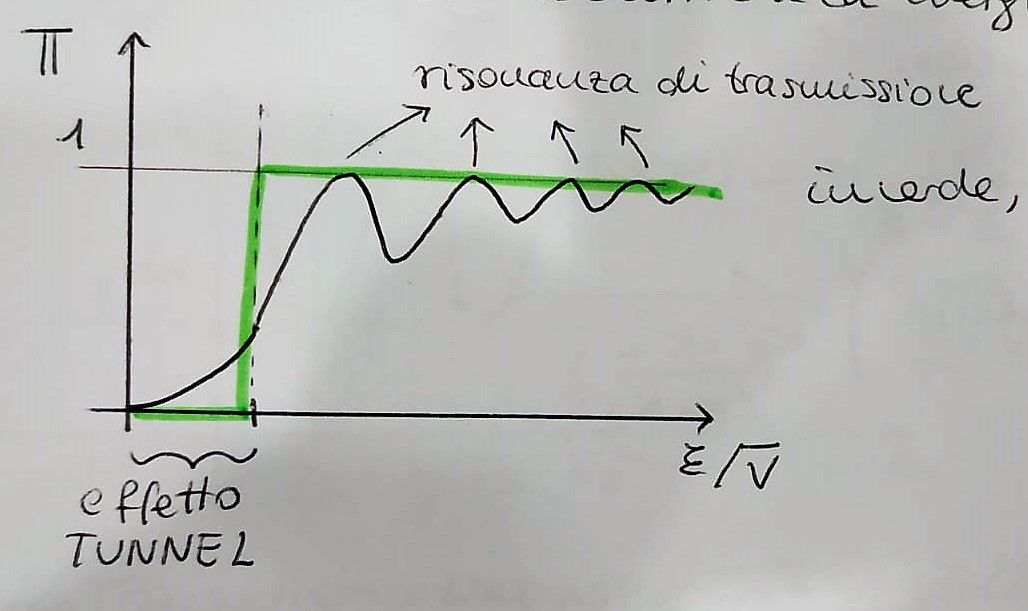
\includegraphics[scale=0.4]{Immagini/TEbassa.jpeg}
%\caption{$\bb{T}(\mathcal{E}/\bar{V})$}
%\end{figure}

\paragraph{Applicazioni del potenziale rettangolare\\}
Il sistema\marginpar{Esempi di utilizzo del potenziale rettangolare} costituito da una particella quantistica che si scontra contro un potenziale rettangolare è un modello ideale che, nella sua semplicità, può spiegare qualitativamente fenomeni ben più complessi, e ha applicazioni in tecniche avanzate di rilevazione. Facciamo qualche esempio.
\begin{itemize}
\item 
\textbf{Radioattività} Consideriamo un nucleo di uranio $^{238}_{92}\mathrm{U}$, dove i due\marginpar{Range dei tempi di decadimento $\alpha$} numeretti ad apice e pedice indicano rispettivamente il numero di nucleoni e di protoni:
\[
^{\overbrace{238}^{\#nucleoni}}_{\underbrace{92}_{\#protoni}}\mathrm{U}
\]
Sperimentalmente si trova che tale atomo decade spontaneamente secondo la reazione:
\[
^{238}_{92}\mathrm{U} \to ^{234}_{90}\mathrm{Th}+\underbrace{\alpha}_{^4_2 \mathrm{He}}
\]
%[IMMAGINE] modello del potenziale centrale dell'atomo: coulombiano oltre al raggio del nucleo $R$ (decresce come 1/r), e buca di potenziale all'interno.
Ossia, spontaneamente, una coppia di protoni e neutroni \q{si libera} dal nucleo.\\
Possiamo schematizzare il nucleo come una \textit{buca di potenziale} molto profonda rispetto al \textit{potenziale coulombiano} che vi è attorno ad essa\footnote{Ciò si ha poiché l'interazione nucleare forte è \q{molto più forte} dell'interazione elettromagnetica, ma è anche a corto raggio, mentre quest'ultima ha raggio infinito.}.\\
La differenza di energia tra il fondo della buca e l'esterno è dell'ordine di \SI{25}{\mega\eV}.\\
In questa buca si trovano i nucleoni. Poiché, prima o poi, una particella $\alpha$ si libera dal nucleo, la sua funzione d'onda all'esterno oscilla all'infinito, e quindi tale $\varphi_\mathcal{E} \notin \hs$, per cui gli autovalori $\mathcal{E}$ di $H$ delle soluzioni \textit{uscenti} devono appartenere allo spettro continuo di $H$: $\mathcal{E}\in \sigma_C(H)$.\\
Perciò una particella all'interno del nucleo si comporta come un \textit{pacchetto d'onda} (in analogia a quanto visto nell'esempio), che ha un'energia concentrata attorno ad un certo valore $\mathcal{E}_0$, che si può misurare sperimentalmente una volta che tale particella è uscita dal nucleo e si trova sufficientemente lontana da ogni sorgente di campi elettrici. Da queste misure scopriamo che il salto tra $\mathcal{E}_0$ e il potenziale esterno è in generale dell'ordine di \num{4}-\SI{9}{\mega\eV}. Tale range relativamente piccolo deve però spiegare l'estrema varietà di \textit{tempi di decadimento}, che vanno dai $10^{-7}$\si{\s}, ai $10^{10}$ anni. Ci aspettiamo quindi che una \textit{piccola} variazione nel dislivello tra $\mathcal{E}_0$ e $\bar{V}$ provochi una \textit{grandissima} variazione nella \textit{probabilità} di uscita dal nucleo: e ciò è proprio quello che si nota osservando la formula (\ref{eqn:effetto_tunnel}) e l'andamento \textit{esponenziale} di tale probabilità in funzione del dislivello energetico.

 \item \textbf{Microscopio a effetto tunnel} (STM:\ Scanning Tunnelling Microscope).\marginpar{Microscopio a effetto tunnel}\\
\begin{figure}[H]
\centering

\tikzset{every picture/.style={line width=0.75pt}} %set default line width to 0.75pt        

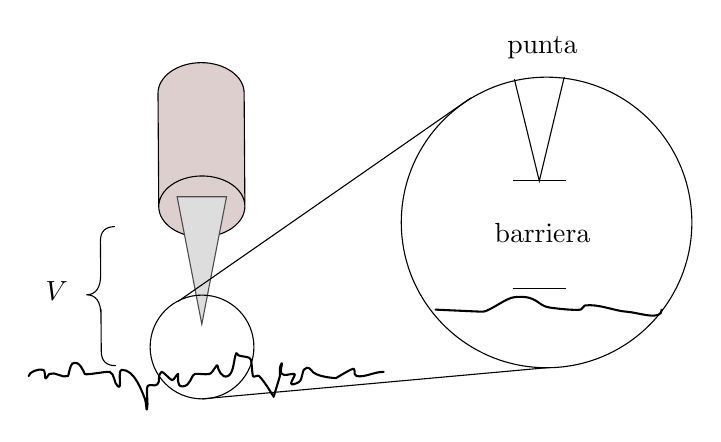
\begin{tikzpicture}[x=0.75pt,y=0.75pt,yscale=-1,xscale=1]
%uncomment if require: \path (0,382); %set diagram left start at 0, and has height of 382

%Flowchart: Magnetic Disk [id:dp14259843128474814] 
\draw  [fill={rgb, 255:red, 201; green, 178; blue, 178 }  ,fill opacity=0.62 ] (197.15,175.44) -- (196.79,120.85) .. controls (196.74,112.73) and (205.99,106.09) .. (217.44,106.01) .. controls (228.9,105.94) and (238.24,112.46) .. (238.29,120.57) -- (238.65,175.16)(197.15,175.44) .. controls (197.1,167.32) and (206.35,160.68) .. (217.81,160.6) .. controls (229.27,160.53) and (238.6,167.05) .. (238.65,175.16) .. controls (238.71,183.28) and (229.46,189.92) .. (218,190) .. controls (206.54,190.07) and (197.21,183.55) .. (197.15,175.44) -- cycle ;
%Flowchart: Merge [id:dp575803647297134] 
\draw  [color={rgb, 255:red, 77; green, 77; blue, 77 }  ,draw opacity=1 ][fill={rgb, 255:red, 221; green, 221; blue, 221 }  ,fill opacity=1 ] (206,170.6) -- (229.81,170.6) -- (217.9,232) -- cycle ;
%Shape: Free Drawing [id:dp7653232054226127] 
\draw  [color={rgb, 255:red, 0; green, 0; blue, 0 }  ][line width=0.75] [line join = round][line cap = round] (134.5,257) .. controls (134.5,255.12) and (139.3,253.27) .. (141.5,254) .. controls (142.5,254.33) and (142.14,256.92) .. (142.5,258) .. controls (142.8,258.89) and (143.66,256.42) .. (144.5,256) .. controls (147.2,254.65) and (150.73,258.19) .. (153.5,257) .. controls (153.57,256.97) and (154.53,251.48) .. (155.5,251) .. controls (159,249.25) and (160.75,254.5) .. (161.5,256) .. controls (161.87,256.74) and (172.3,254.6) .. (173.5,255) .. controls (176.05,255.85) and (175.35,260.39) .. (177.5,262) .. controls (179.85,263.77) and (176.88,254) .. (179.5,254) .. controls (185.56,254) and (189.02,264.41) .. (190.5,268) .. controls (191.15,269.57) and (191.17,274.67) .. (191.5,273) .. controls (192.15,269.73) and (191.2,266.32) .. (191.5,263) .. controls (191.81,259.63) and (194.9,262.6) .. (196.5,261) .. controls (198.18,259.32) and (196.04,257.46) .. (198.5,255) .. controls (198.95,254.55) and (202.4,258.45) .. (203.5,259) .. controls (204.29,259.4) and (206.33,255.32) .. (206.5,256) .. controls (206.7,256.78) and (205.42,262) .. (208.5,262) .. controls (212.64,262) and (212.85,256.24) .. (214.5,256) .. controls (216.81,255.67) and (219.21,256.46) .. (221.5,256) .. controls (223.35,255.63) and (225.5,250.11) .. (225.5,252) .. controls (225.5,253.41) and (227.52,258.49) .. (230.5,257) .. controls (233.48,255.51) and (233.2,248.6) .. (234.5,246) .. controls (234.71,245.58) and (235.11,246.74) .. (235.5,247) .. controls (236.6,247.73) and (241.11,247.43) .. (241.5,249) .. controls (242.15,251.61) and (241.97,254.36) .. (242.5,257) .. controls (242.7,257.98) and (244.79,256.29) .. (245.5,257) .. controls (248.38,259.88) and (252.5,267) .. (252.5,267) .. controls (252.5,267) and (255.38,257.69) .. (255.5,257) .. controls (255.72,255.68) and (255.24,254.31) .. (255.5,253) .. controls (255.65,252.27) and (256.5,250.25) .. (256.5,251) .. controls (256.5,252.67) and (255.22,254.93) .. (256.5,256) .. controls (258.04,257.28) and (260.53,255.67) .. (262.5,256) .. controls (263.98,256.25) and (256.96,263.77) .. (264.5,260) .. controls (266.9,258.8) and (265.81,253) .. (268.5,253) .. controls (269.25,253) and (270.17,253.33) .. (270.5,254) .. controls (272.3,257.59) and (282.5,258) .. (282.5,258) .. controls (282.5,258) and (287.95,254.77) .. (289.5,254) .. controls (293.31,252.1) and (290.05,256.51) .. (292.5,257) .. controls (296.45,257.79) and (300.57,255) .. (305.5,255) ;
%Shape: Brace [id:dp3527177890628157] 
\draw   (176,185) .. controls (171.33,185.03) and (169.02,187.38) .. (169.05,192.05) -- (169.17,207.8) .. controls (169.22,214.47) and (166.92,217.82) .. (162.25,217.86) .. controls (166.92,217.82) and (169.27,221.13) .. (169.32,227.8)(169.3,224.8) -- (169.45,245.05) .. controls (169.48,249.72) and (171.83,252.03) .. (176.5,252) ;
%Shape: Circle [id:dp46797943083352833] 
\draw   (193,243) .. controls (193,229.19) and (204.19,218) .. (218,218) .. controls (231.81,218) and (243,229.19) .. (243,243) .. controls (243,256.81) and (231.81,268) .. (218,268) .. controls (204.19,268) and (193,256.81) .. (193,243) -- cycle ;
%Shape: Circle [id:dp14383965272185373] 
\draw   (314,183) .. controls (314,144.34) and (345.34,113) .. (384,113) .. controls (422.66,113) and (454,144.34) .. (454,183) .. controls (454,221.66) and (422.66,253) .. (384,253) .. controls (345.34,253) and (314,221.66) .. (314,183) -- cycle ;
%Straight Lines [id:da8052490977028961] 
\draw    (347.5,123) -- (206.5,221) ;

%Straight Lines [id:da6765015408756323] 
\draw    (384,253) -- (218,268) ;

%Shape: Free Drawing [id:dp25298029912790243] 
\draw  [color={rgb, 255:red, 0; green, 0; blue, 0 }  ][line width=0.75] [line join = round][line cap = round] (330.5,225) .. controls (330.73,225) and (353.14,226.06) .. (353.5,226) .. controls (357.35,225.3) and (364.41,219.41) .. (368.5,219) .. controls (379.88,217.86) and (379.18,223.1) .. (385.5,224) .. controls (388.9,224.49) and (397.25,225.46) .. (400.5,225) .. controls (401.43,224.87) and (401.57,223.13) .. (402.5,223) .. controls (408.85,222.09) and (416.96,225.67) .. (422.5,226) .. controls (428.17,226.33) and (439.5,230.68) .. (439.5,225) ;
%Straight Lines [id:da9828628896091545] 
\draw    (368.5,114) -- (380.5,163) -- (392.5,113) ;

%Straight Lines [id:da9772593884211451] 
\draw    (367.75,163) -- (393.25,163) ;

%Straight Lines [id:da6724181640842126] 
\draw    (367.75,215) -- (393.25,215) ;

% Text Node
\draw (148,216) node   {$V$};
% Text Node
\draw (382,99) node  [align=left] {punta};
% Text Node
\draw (382,188) node  [align=left] {barriera};
\end{tikzpicture}
\caption{Schema del microscopio a effetto tunnel}
\end{figure}

Si può sfruttare l'effetto tunnel per ottenere microscopi sensibilissimi.\\
Consideriamo una punta conduttrice molto fine (di poche decine di atomi di larghezza), che viene avvicinata all'oggetto in esame.\\
Si applica una differenza di potenziale tra materiale (ricoperto di un sottile strato conduttore) e punta del microscopio. Si avvicina la punta al materiale, lasciando un certo spazio vuoto tra essa e la superficie. Tale distanza funge da \textit{barriera di potenziale}: classicamente gli elettroni dell'oggetto rimarrebbero sull'oggetto, e quelli della punta sulla punta.\\
Tuttavia, per effetto tunnel, c'è una probabilità che gli elettroni passino dalla superficie alla punta, generando una corrente che può essere misurata.\\
Supponiamo ora di muovere la punta in modo da mantenere questa corrente \textit{di tunnel} costante: per farlo dovremo periodicamente avvicinare o allontanare la punta stessa, a seconda delle caratteristiche della superficie in esame. Otteniamo perciò una procedura per mappare le aree del materiale a densità di carica costante (\textit{local density of states} - LDOS). Individuiamo quindi la \q{nuvola di carica} elettronica, e misurandola possiamo, in un certo senso, \q{vedere} gli atomi.
\end{itemize}
\end{document}
